\documentclass[12pt, a4paper]{article}\usepackage[]{graphicx}\usepackage[]{color}
%% maxwidth is the original width if it is less than linewidth
%% otherwise use linewidth (to make sure the graphics do not exceed the margin)
\makeatletter
\def\maxwidth{ %
  \ifdim\Gin@nat@width>\linewidth
    \linewidth
  \else
    \Gin@nat@width
  \fi
}
\makeatother

\definecolor{fgcolor}{rgb}{0.345, 0.345, 0.345}
\newcommand{\hlnum}[1]{\textcolor[rgb]{0.686,0.059,0.569}{#1}}%
\newcommand{\hlstr}[1]{\textcolor[rgb]{0.192,0.494,0.8}{#1}}%
\newcommand{\hlcom}[1]{\textcolor[rgb]{0.678,0.584,0.686}{\textit{#1}}}%
\newcommand{\hlopt}[1]{\textcolor[rgb]{0,0,0}{#1}}%
\newcommand{\hlstd}[1]{\textcolor[rgb]{0.345,0.345,0.345}{#1}}%
\newcommand{\hlkwa}[1]{\textcolor[rgb]{0.161,0.373,0.58}{\textbf{#1}}}%
\newcommand{\hlkwb}[1]{\textcolor[rgb]{0.69,0.353,0.396}{#1}}%
\newcommand{\hlkwc}[1]{\textcolor[rgb]{0.333,0.667,0.333}{#1}}%
\newcommand{\hlkwd}[1]{\textcolor[rgb]{0.737,0.353,0.396}{\textbf{#1}}}%
\let\hlipl\hlkwb

\usepackage{framed}
\makeatletter
\newenvironment{kframe}{%
 \def\at@end@of@kframe{}%
 \ifinner\ifhmode%
  \def\at@end@of@kframe{\end{minipage}}%
  \begin{minipage}{\columnwidth}%
 \fi\fi%
 \def\FrameCommand##1{\hskip\@totalleftmargin \hskip-\fboxsep
 \colorbox{shadecolor}{##1}\hskip-\fboxsep
     % There is no \\@totalrightmargin, so:
     \hskip-\linewidth \hskip-\@totalleftmargin \hskip\columnwidth}%
 \MakeFramed {\advance\hsize-\width
   \@totalleftmargin\z@ \linewidth\hsize
   \@setminipage}}%
 {\par\unskip\endMakeFramed%
 \at@end@of@kframe}
\makeatother

\definecolor{shadecolor}{rgb}{.97, .97, .97}
\definecolor{messagecolor}{rgb}{0, 0, 0}
\definecolor{warningcolor}{rgb}{1, 0, 1}
\definecolor{errorcolor}{rgb}{1, 0, 0}
\newenvironment{knitrout}{}{} % an empty environment to be redefined in TeX

\usepackage{alltt}
\usepackage[utf8]{inputenc}
\usepackage{longtable}
\usepackage{multirow} 
\usepackage{hyperref}
\usepackage[titles]{tocloft}
\usepackage[affil-it]{authblk}
\usepackage{geometry}
\geometry{verbose,tmargin=3cm,bmargin=3cm,lmargin=3cm,rmargin=3cm}

\setlength\parindent{0pt}

\title{\textbf{\Large Alignment Stats}}

\author {Lucas Michel Todó, Cristina Bancells\\
Alfred Cortes and Juan R. Gonzalez}

\affil{Barcelona Global Health Institute (ISGlobal), Campus PRBB}
\IfFileExists{upquote.sty}{\usepackage{upquote}}{}
\begin{document}

\maketitle
\tableofcontents
\newpage



\section{Params}
Params 1: -p 1 --very-sensitive --local -5 4 -3 4 -I 50 -X 250 \\
Params 2: -p 1 --very-sensitive --local -5 4 -3 4 -I 50 -X 10000 \\
Params 3: -p 1 --very-sensitive --local -5 12 -3 4 -I 50 -X 10000 \\
Params 4: -p 1 --very-sensitive --local -N 1 -5 12 -3 4 -I 50 -X 10000 \\




\section{Tables}



\subsection{Stats}
\begin{knitrout}\tiny
\definecolor{shadecolor}{rgb}{0.969, 0.969, 0.969}\color{fgcolor}\begin{kframe}
\begin{alltt}
\hlkwd{print}\hlstd{(params)}
\end{alltt}
\begin{verbatim}
##                              Stats  A7li__1  E5li__1  A7li__2  E5li__2  A7li__3  E5li__3  A7li__4  E5li__4
## 1             raw total sequences:   110000   110000   110000   110000   110000   110000   110000   110000
## 2              filtered sequences:        0        0        0        0        0        0        0        0
## 3                       sequences:   110000   110000   110000   110000   110000   110000   110000   110000
## 4                       is sorted:        0        0        0        0        0        0        0        0
## 5                   1st fragments:    55000    55000    55000    55000    55000    55000    55000    55000
## 6                  last fragments:    55000    55000    55000    55000    55000    55000    55000    55000
## 7                    reads mapped:   107246   103551   107254   103562   107242   103725   107242   103725
## 8         reads mapped and paired:   106860   102230   106876   102252   106852   102280   106852   102280
## 10                 reads unmapped:     2754     6449     2746     6438     2758     6275     2758     6275
## 11          reads properly paired:    83696    80930    92538    89960    86150    84542    86150    84542
## 13                   reads paired:   110000   110000   110000   110000   110000   110000   110000   110000
## 15               reads duplicated:        0        0        0        0        0        0        0        0
## 17                      reads MQ0:      569      837      551      862      755      983      755      983
## 19                reads QC failed:        0        0        0        0        0        0        0        0
## 20         non-primary alignments:        0        0        0        0        0        0        0        0
## 21                   total length: 12870000 12870000 12870000 12870000 11990000 11990000 11990000 11990000
## 23                   bases mapped: 12547782 12115467 12548718 12116754 11689378 11306025 11689378 11306025
## 25           bases mapped (cigar): 11949843 11418154 12033129 11499675 11139112 10656163 11139112 10656163
## 27                  bases trimmed:        0        0        0        0        0        0        0        0
## 28               bases duplicated:        0        0        0        0        0        0        0        0
## 29                     mismatches:   146980   142347   142160   136729   124022   121296   124022   121296
## 31                     error rate:        0        0        0        0        0        0        0        0
## 33                 average length:      117      117      117      117      109      109      109      109
## 34                 maximum length:      117      117      117      117      109      109      109      109
## 35                average quality:       35       34       35       34       35       34       35       34
## 36            insert size average:      153      156      185      189      181      186      181      186
## 37 insert size standard deviation:       42       42      121      125      155      162      155      162
## 38          inward oriented pairs:    44729    43407    45504    44180    42242    41497    42242    41497
## 39         outward oriented pairs:     7195     5977     6939     5753    10010     8357    10010     8357
## 40   pairs with other orientation:       64       62       34       32       49       55       49       55
## 41 pairs on different chromosomes:      373      607      134      304      207      377      207      377
\end{verbatim}
\end{kframe}
\end{knitrout}

\subsection{Average Coverage}

\begin{tabular}{l|c|c|c|c|c|c|c|c|c}
\cline{2-9}
&\multicolumn{2}{|c|}{Par 1}&\multicolumn{2}{|c|}{Par 2}&\multicolumn{2}{|c|}{Par 3}&\multicolumn{2}{|c|}{Par 4}\\
\hline
\multicolumn{1}{|l|}{Coding:}&0.593&0.549 &0.595&0.551 &0.550&0.512 &0.550&0.512\\
\hline
\multicolumn{1}{|l|}{Non-Coding:}&0.398&0.373 &0.403&0.378 &0.3670&0.347 &0.3670&0.347\\
\hline
\end{tabular}


\section{Plots}
\subsection{MAPQ}
\noindent


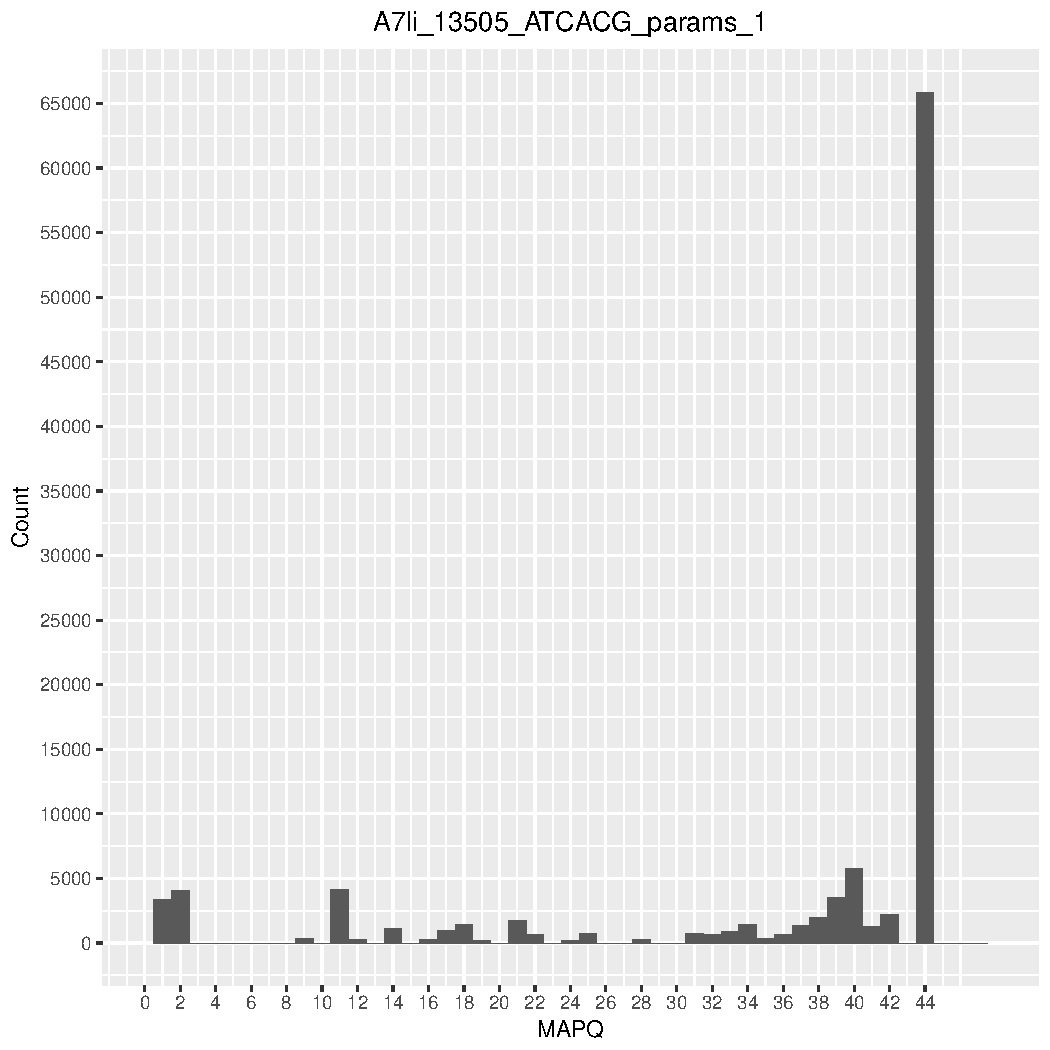
\includegraphics[width=.5\linewidth,height=0.5\textheight]{figure/unnamed-chunk-5-1} 

\includegraphics[width=.5\linewidth,height=0.5\textheight]{figure/unnamed-chunk-5-2} 
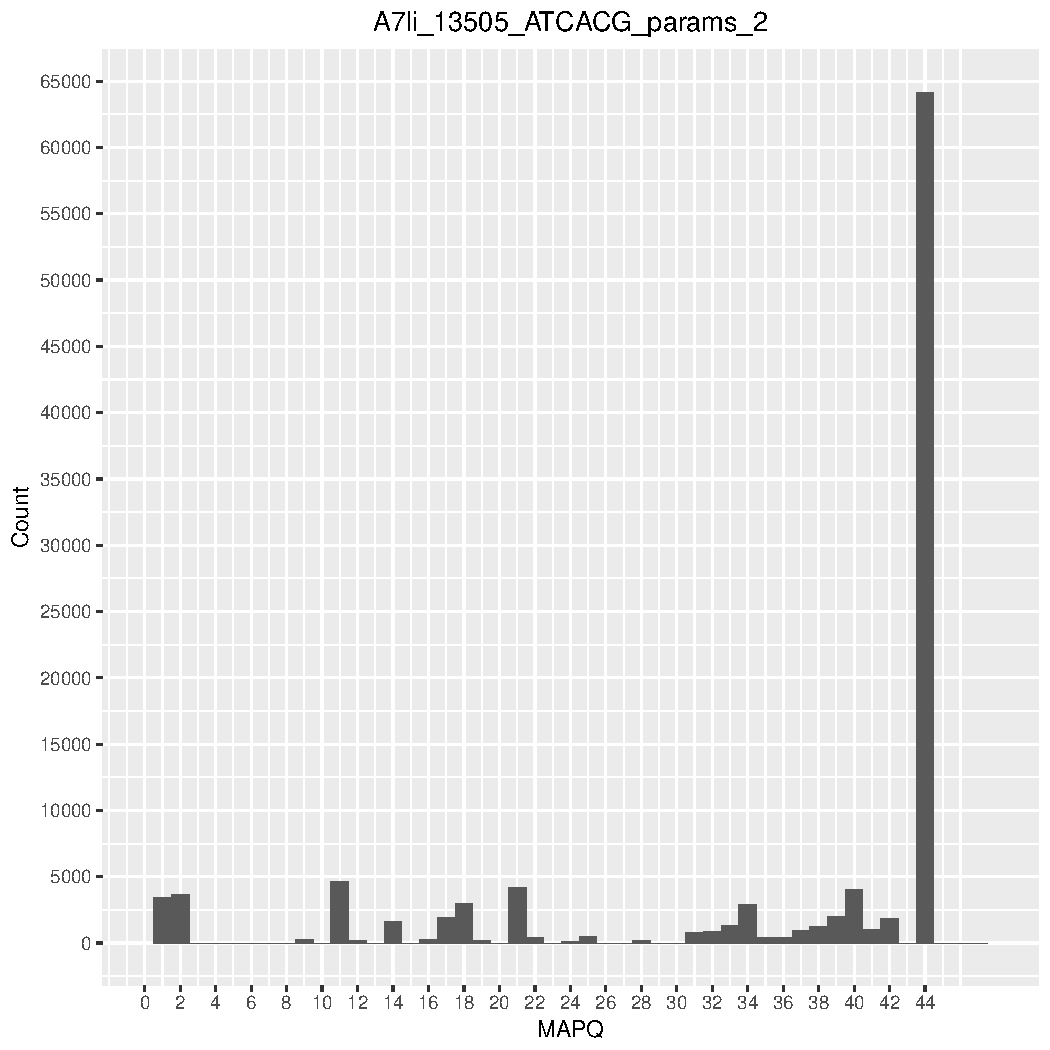
\includegraphics[width=.5\linewidth,height=0.5\textheight]{figure/unnamed-chunk-5-3} 
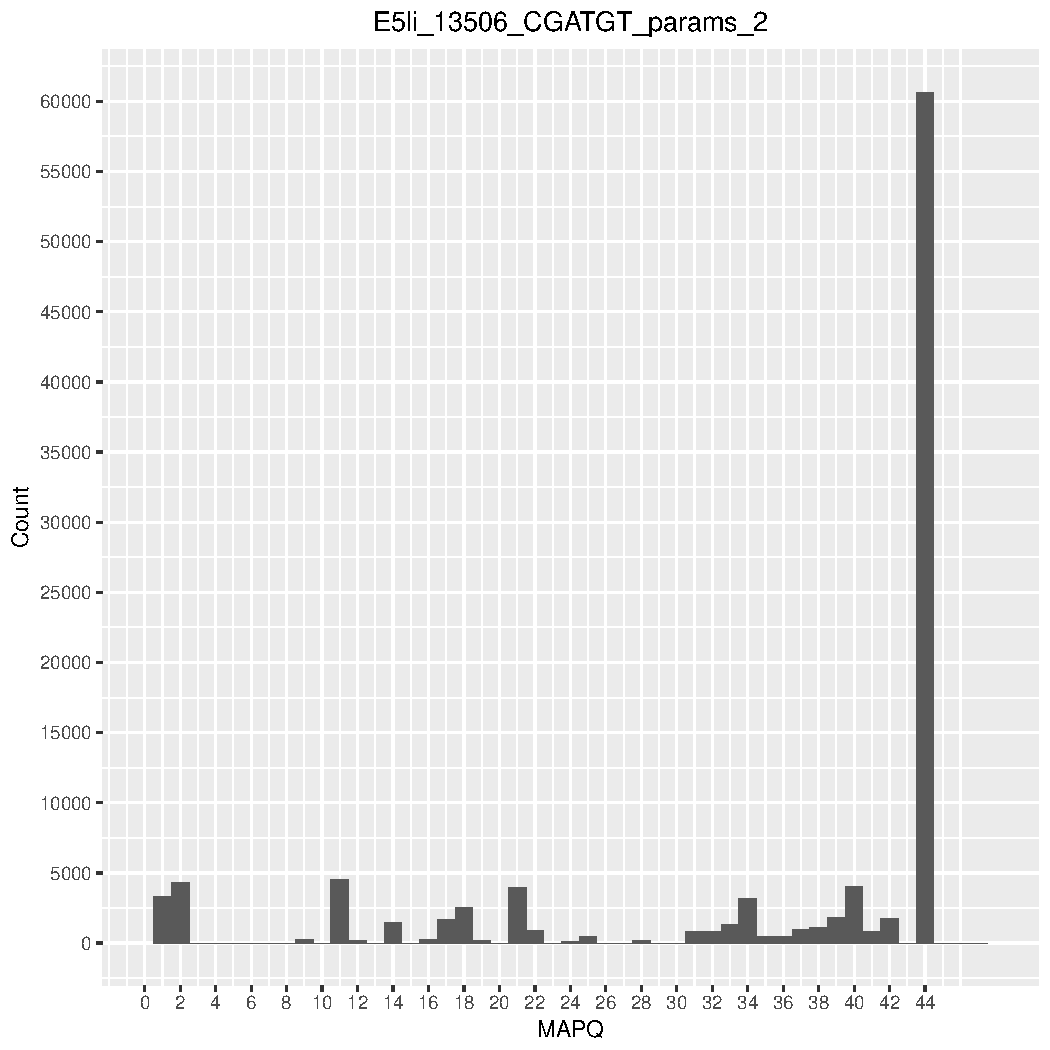
\includegraphics[width=.5\linewidth,height=0.5\textheight]{figure/unnamed-chunk-5-4} 
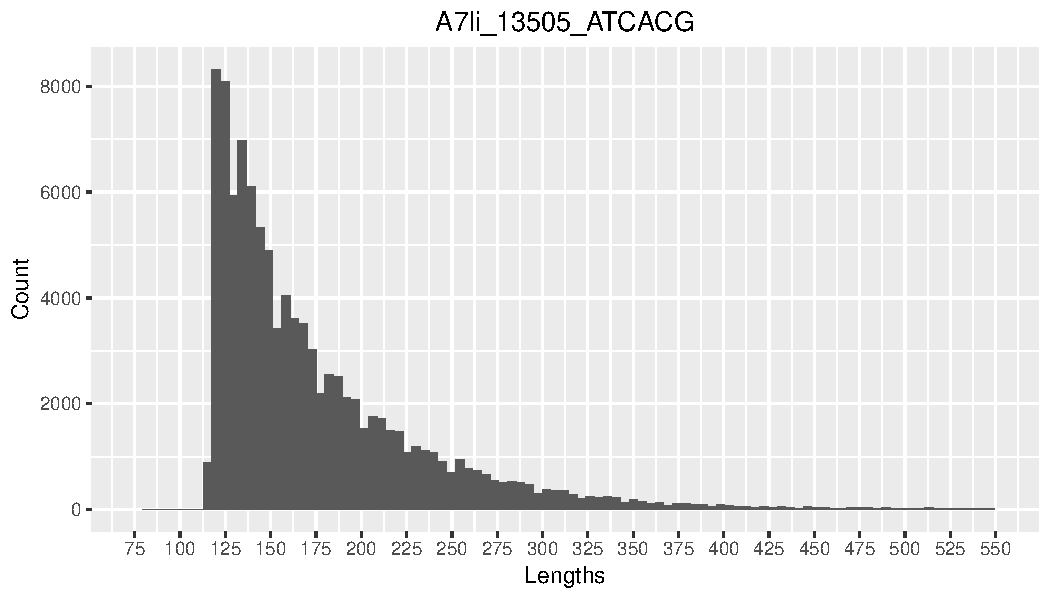
\includegraphics[width=.5\linewidth,height=0.5\textheight]{figure/unnamed-chunk-5-5} 
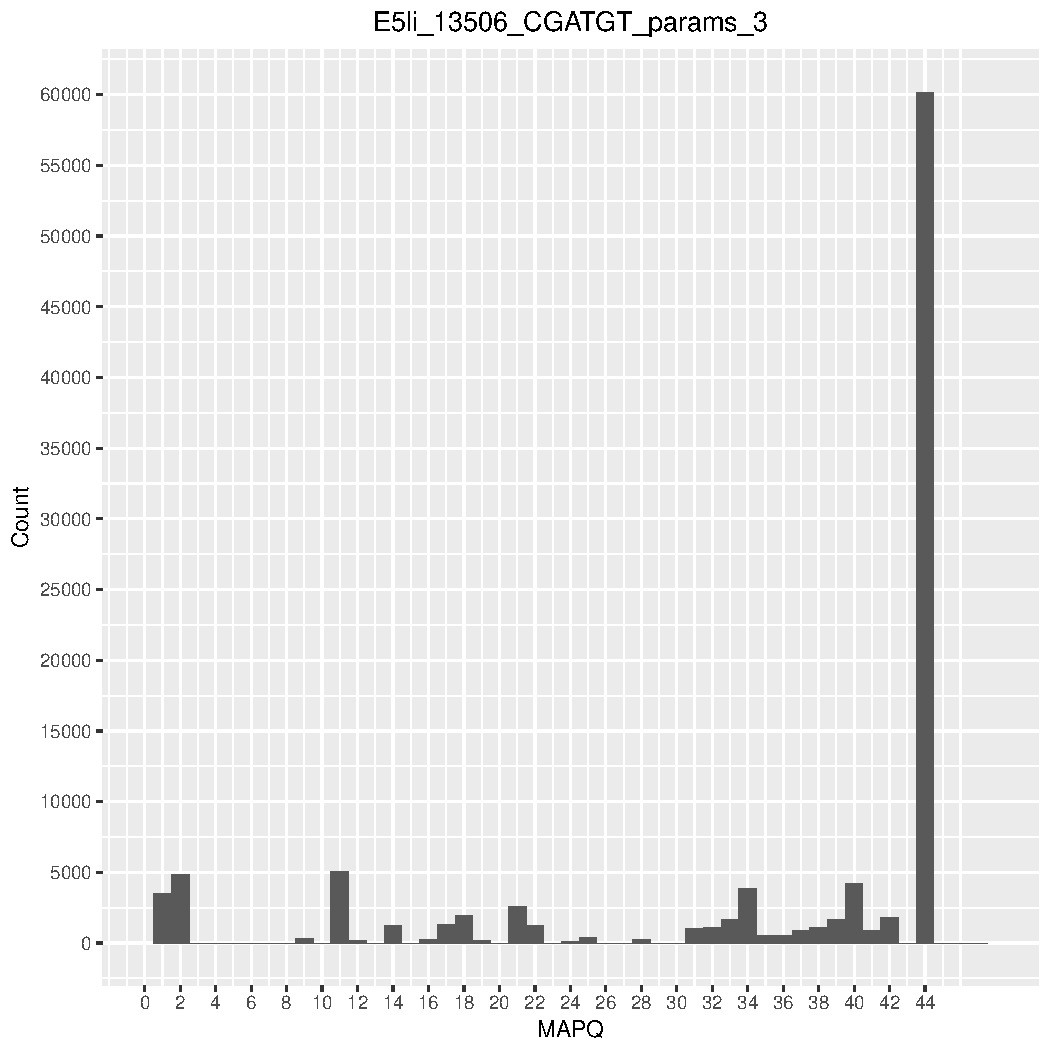
\includegraphics[width=.5\linewidth,height=0.5\textheight]{figure/unnamed-chunk-5-6} 
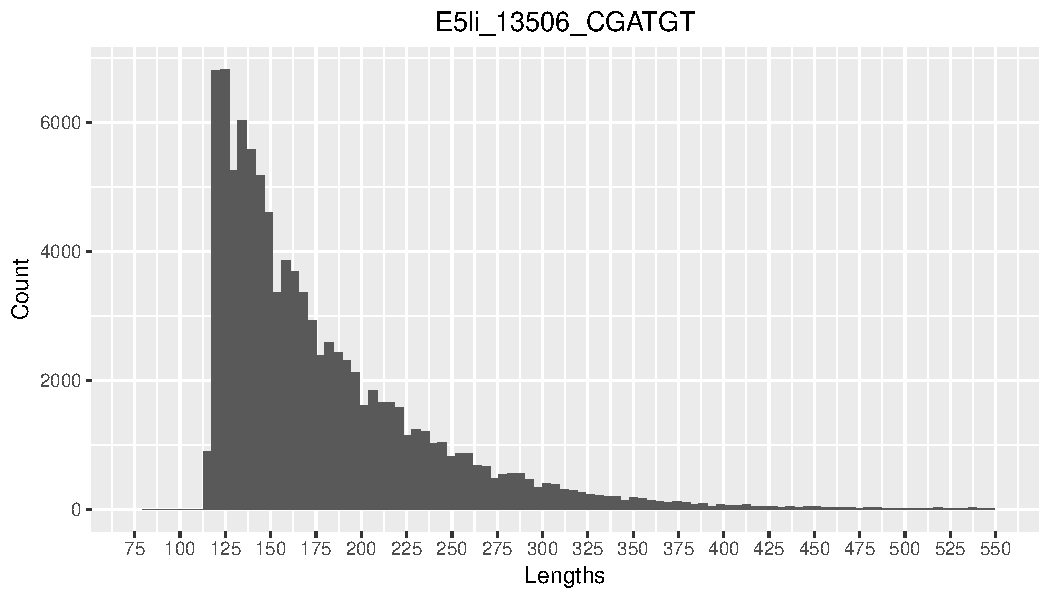
\includegraphics[width=.5\linewidth,height=0.5\textheight]{figure/unnamed-chunk-5-7} 
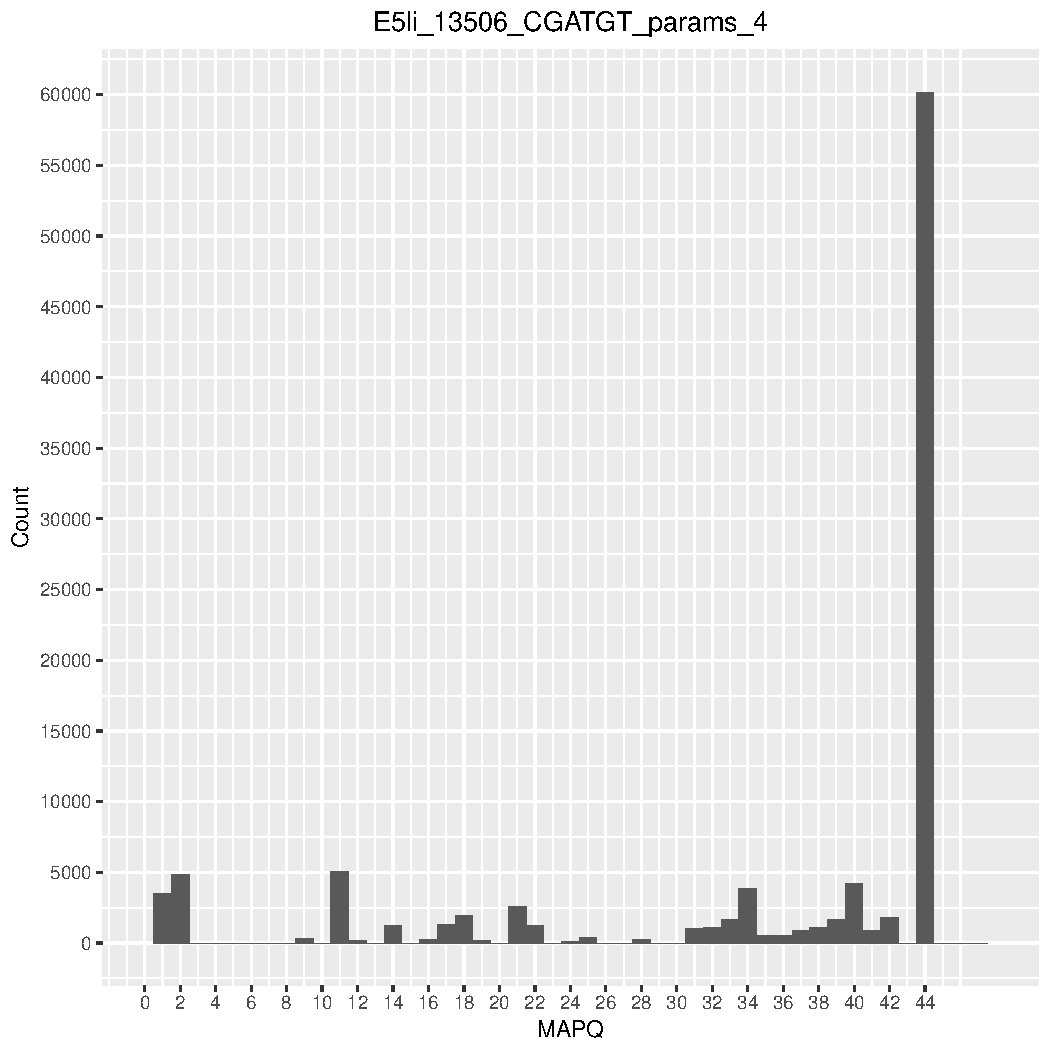
\includegraphics[width=.5\linewidth,height=0.5\textheight]{figure/unnamed-chunk-5-8} 


\clearpage
\subsection{Fragment Length}
\noindent


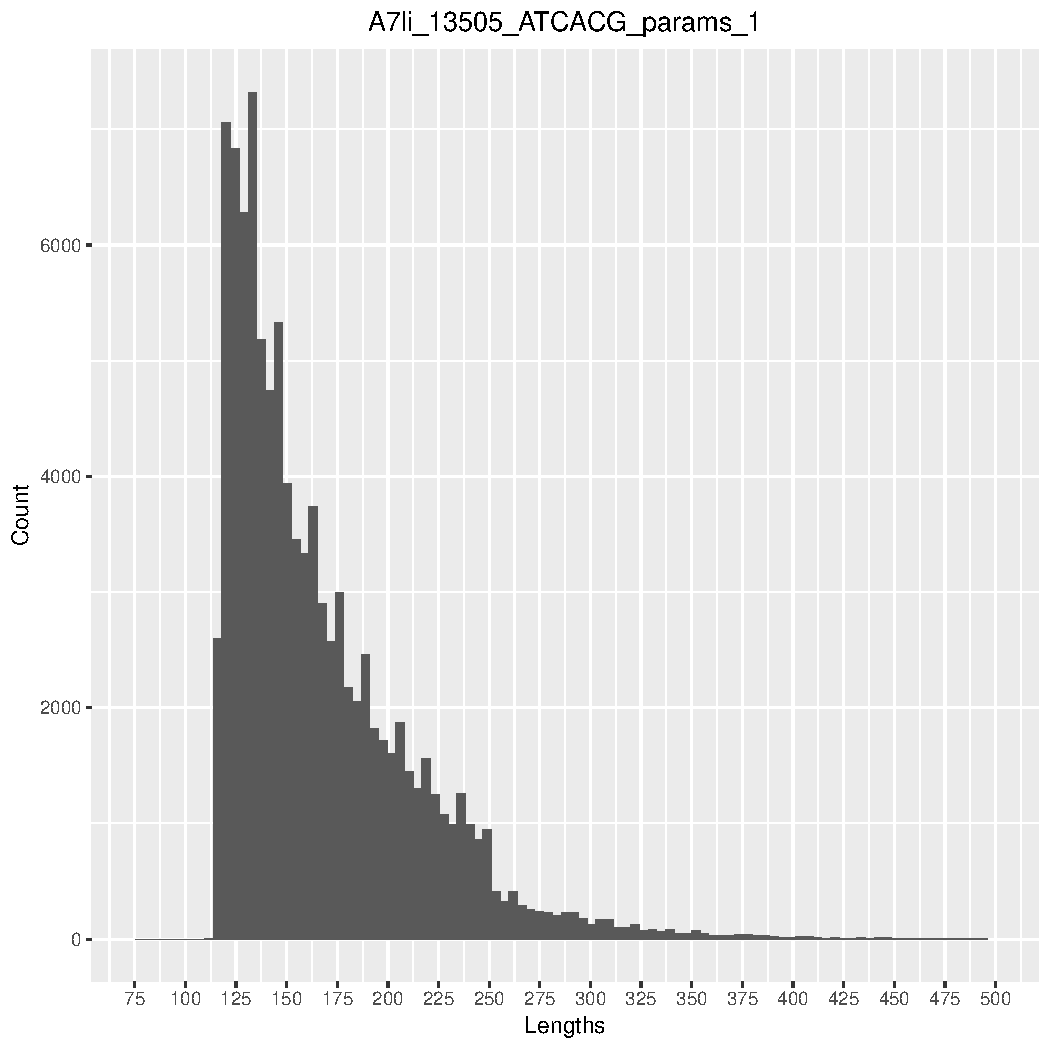
\includegraphics[width=.5\linewidth]{figure/unnamed-chunk-6-1} 
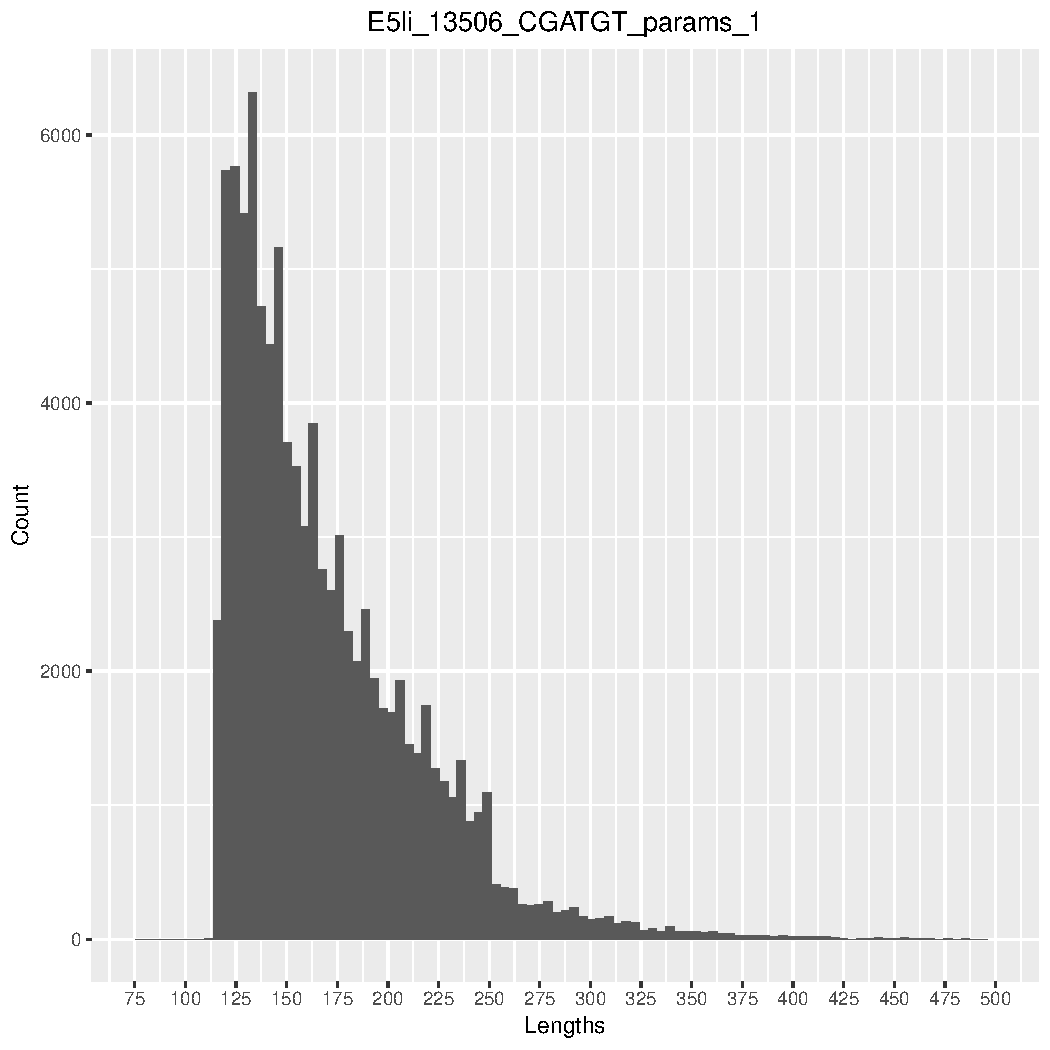
\includegraphics[width=.5\linewidth]{figure/unnamed-chunk-6-2} 
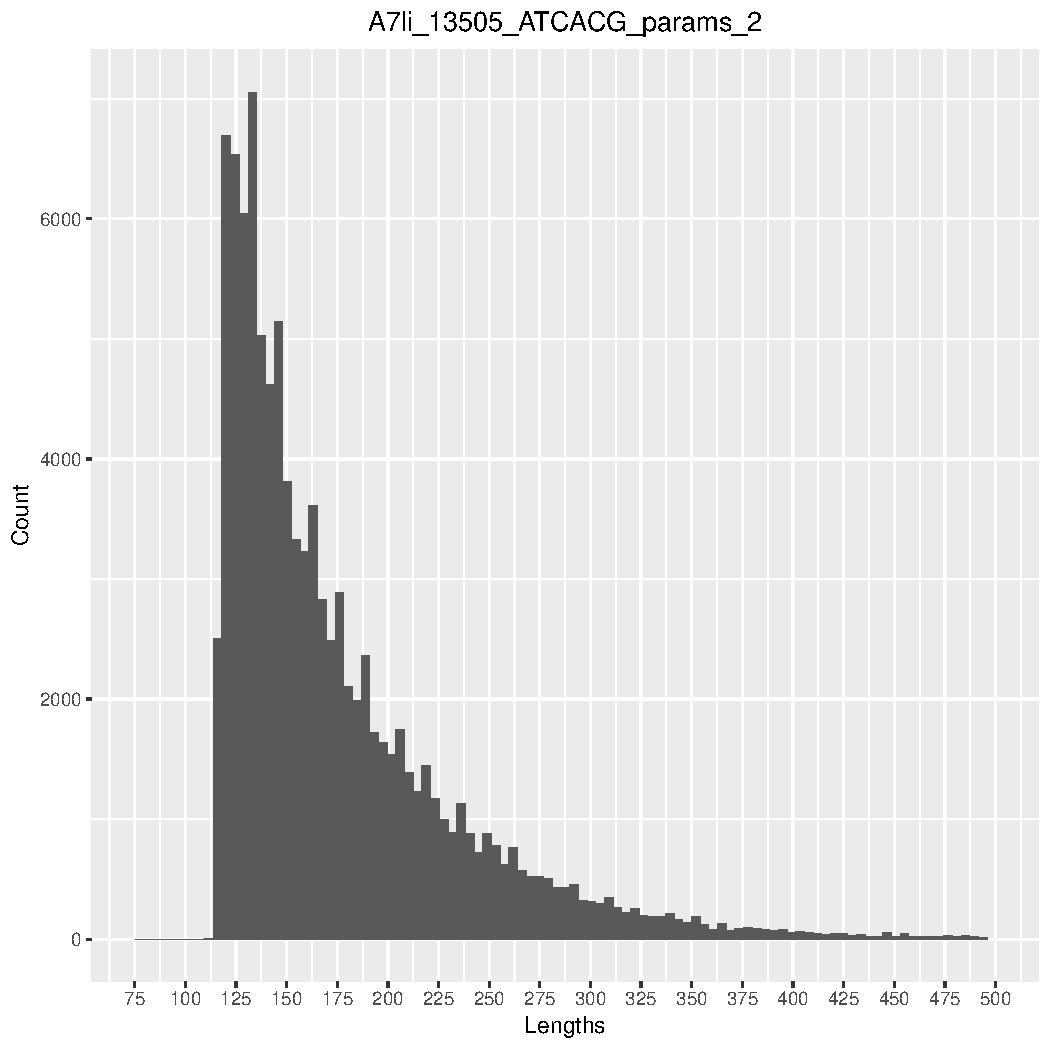
\includegraphics[width=.5\linewidth]{figure/unnamed-chunk-6-3} 
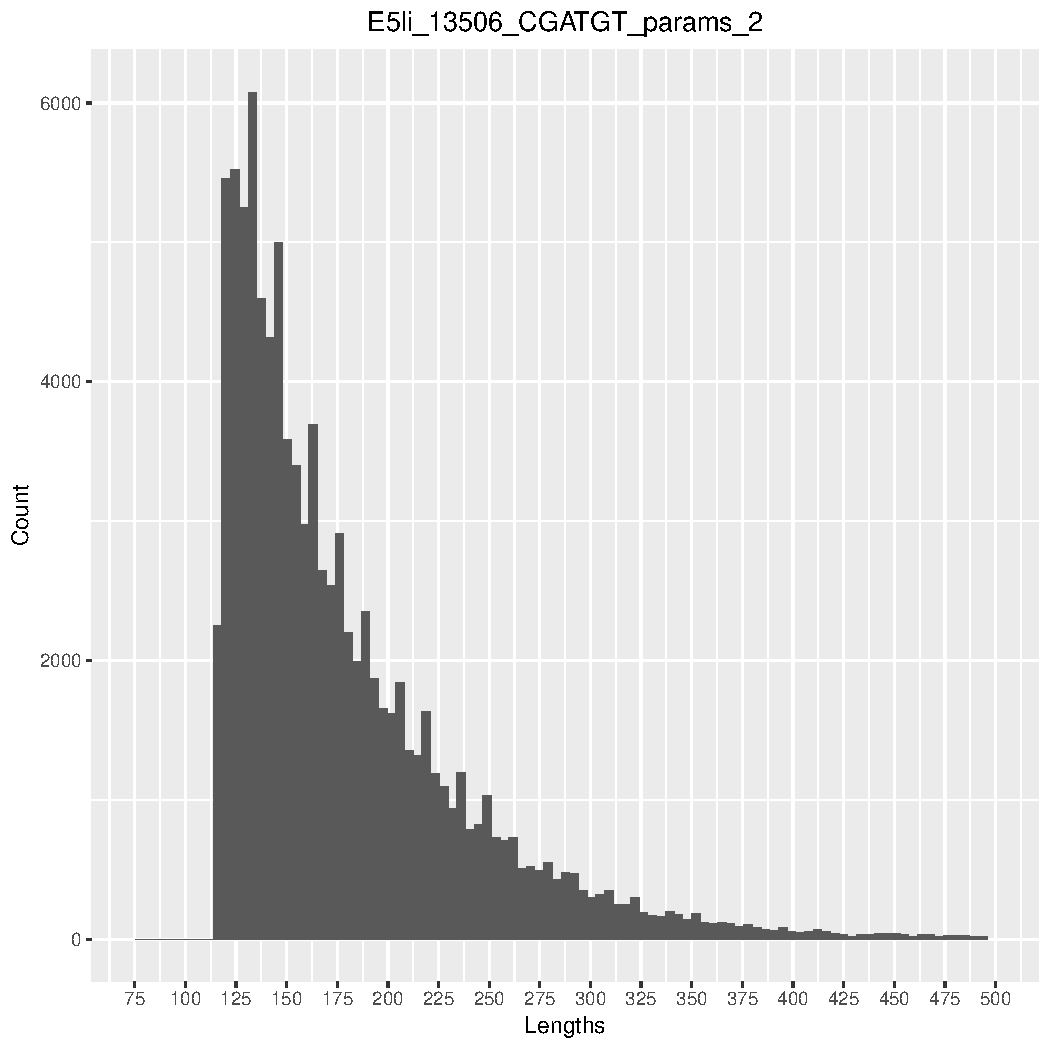
\includegraphics[width=.5\linewidth]{figure/unnamed-chunk-6-4} 
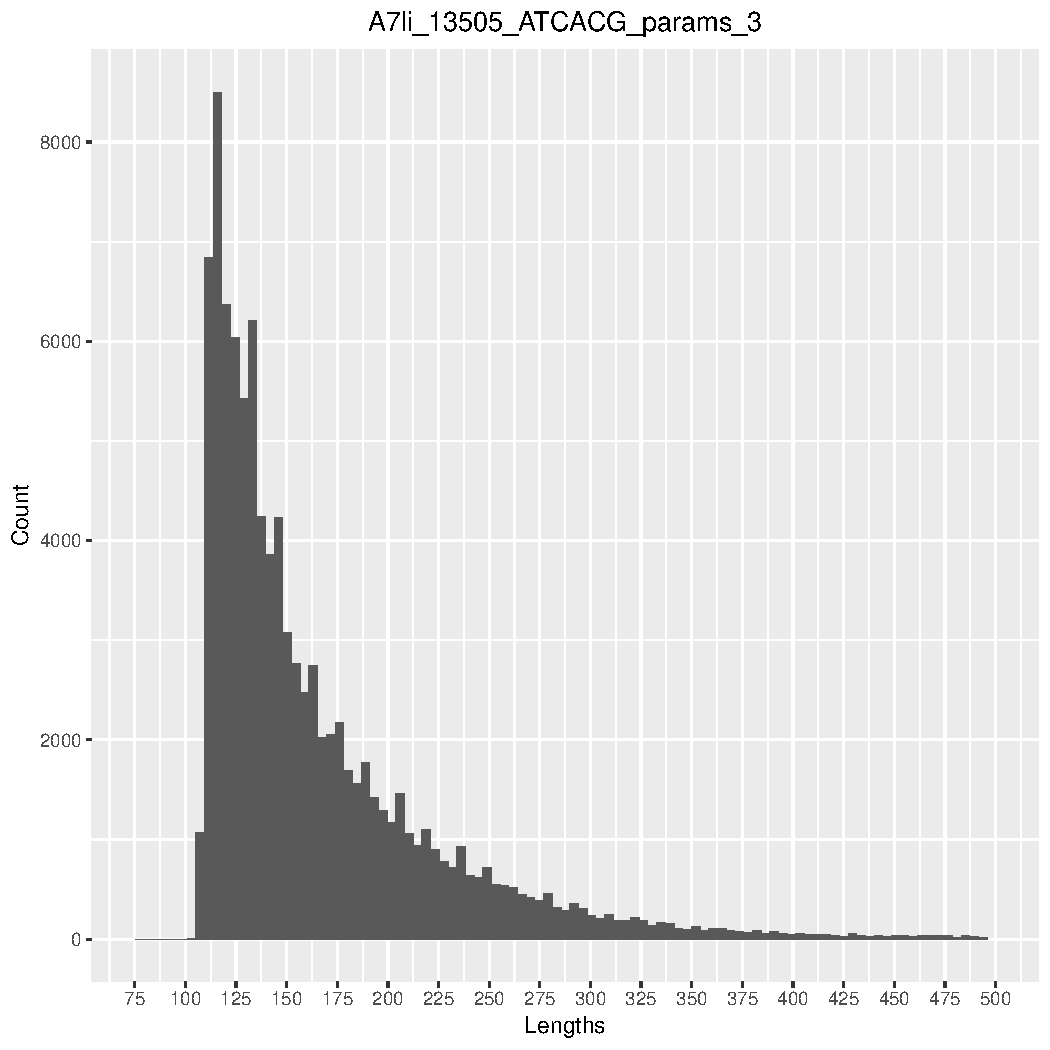
\includegraphics[width=.5\linewidth]{figure/unnamed-chunk-6-5} 
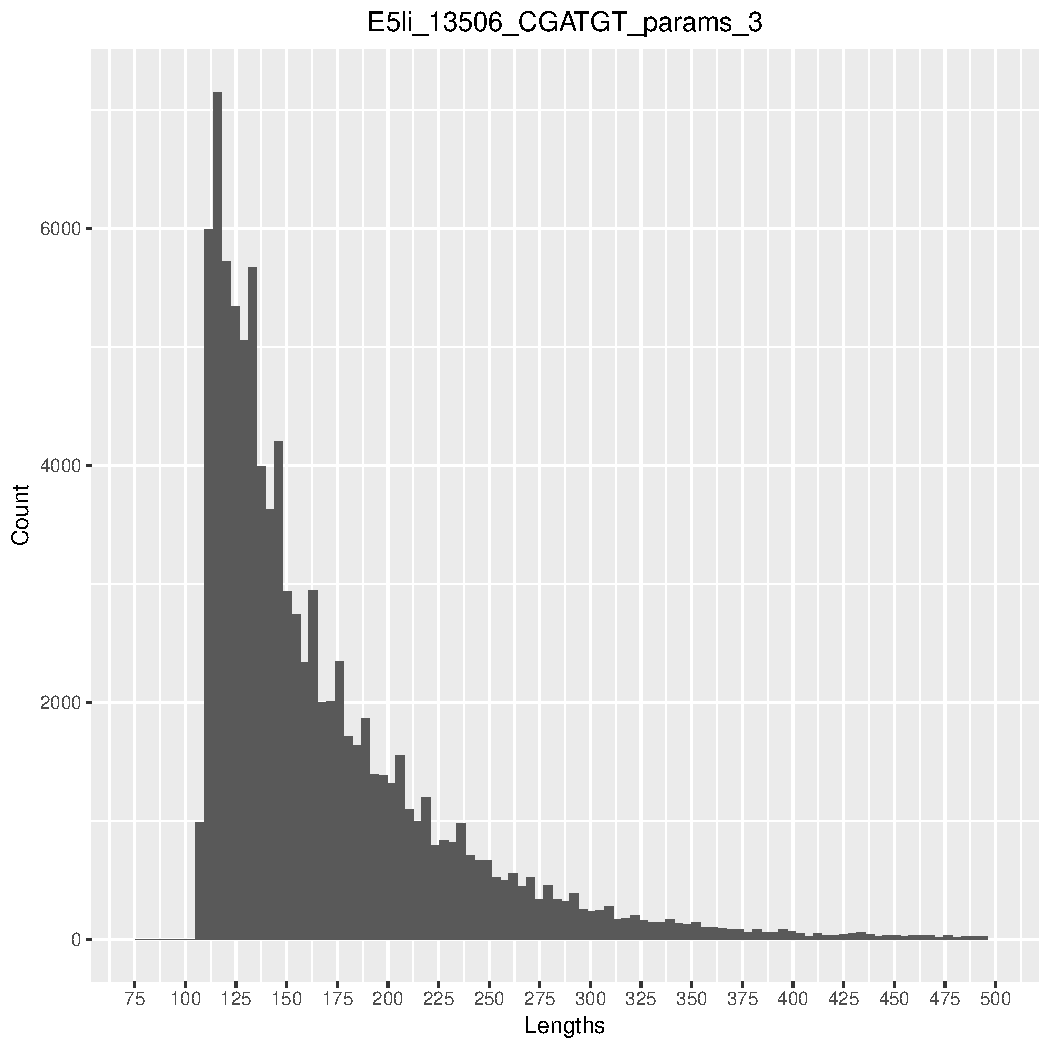
\includegraphics[width=.5\linewidth]{figure/unnamed-chunk-6-6} 
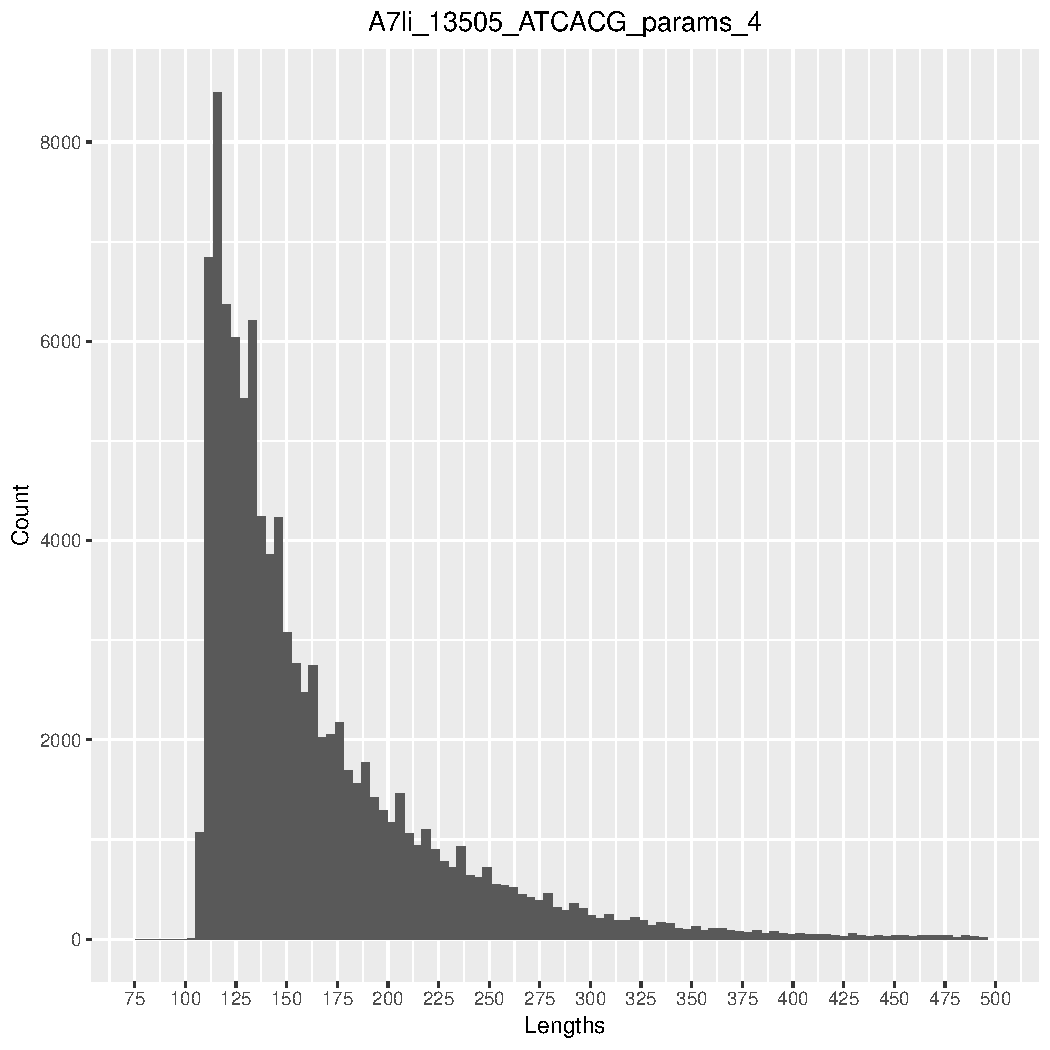
\includegraphics[width=.5\linewidth]{figure/unnamed-chunk-6-7} 
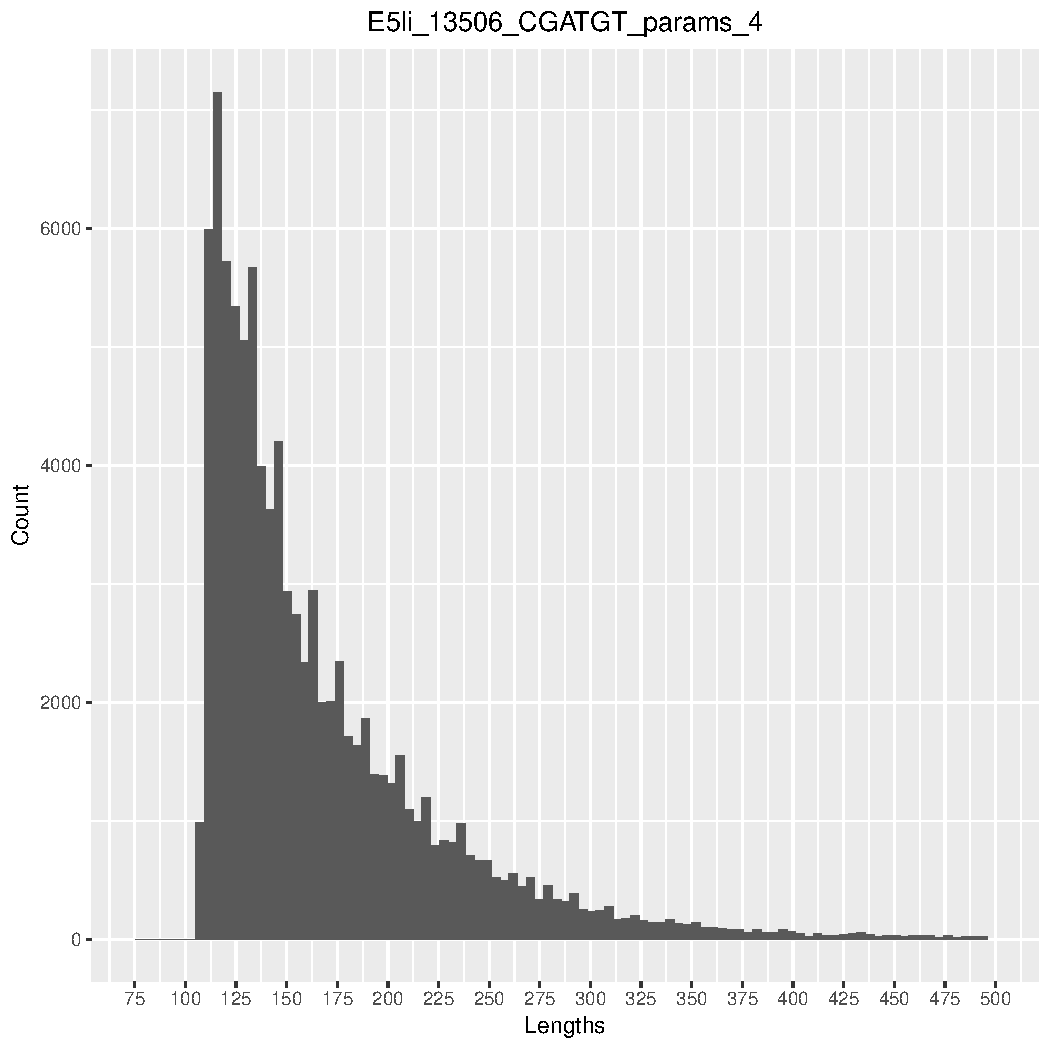
\includegraphics[width=.5\linewidth]{figure/unnamed-chunk-6-8} 


\end{document}
